The \textit{Account} module is responsible for management of users using the system. The scope for the \textit{Account} module is shown in Figure 2.  \\[1cm]

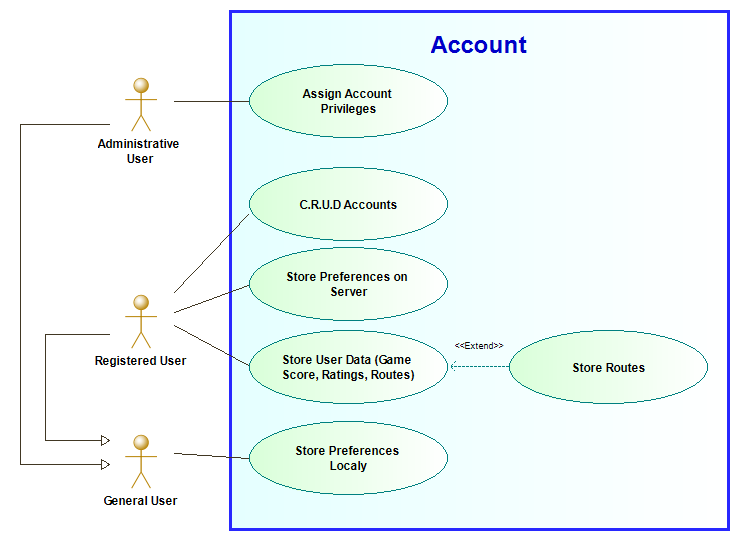
\includegraphics[width=\textwidth]{Account_Use_Case_Diagram}
\begin{center}
	Figure 9: Account Module Use Case
\end{center}

{The account system will allow general users to register themselves and create accounts which will be stored and tracked by the account system. This system will therefore allow users to have access to the rating system, the game system and any other more personalised system provided by the NavUP system as a whole. The account system will allow administrative user to assign user privileges to different accounts. It will also be responsible for storing the users preferences on the server as well as any other data they might enter into the system such as favourite paths and locations as well as routes they have discovered.}
%\begin{enumerate}
%	\item \textbf{Assign Account Privileges}
%	\begin{itemize}
%		\item Description: \\
%		This use case allows the admin user to assign privileges to registered users. He/She may promote or demote users to higher privileges 
%		\item Pre-Conditions: \\
%		\begin{itemize}
%		\item User must be logged in
%		\item User must have admin privileges
%		\item The admin user must supply a registered user in the request
		
%		\end{itemize}
%		\item Post-Conditions: \\
		
%		\begin{itemize}
%		\item The supplied user will have new access privileges 
		
%		\end{itemize}
	
%	\end{itemize}
	
%	\item \textbf{C.R.U.D. Accounts}
%	\begin{itemize}
%		\item Description: \\
%		This use case allow a user to create, update and deactivate an account for the NavUP system
%		\item Pre-Conditions: \\
		
%		\item Post-Conditions: \\
	
%	\end{itemize}
	
%	\item \textbf{Store Preferences on Server}
%	\begin{itemize}
%		\item Description: \\
		
%		\item Pre-Conditions: \\
		
%		\item Post-Conditions: \\
	
%	\end{itemize}
	
%	\item \textbf{Store User Data}
%	\begin{itemize}
%		\item Description: \\
		
%		\item Pre-Conditions: \\
		
%		\item Post-Conditions: \\
	
%	\end{itemize}
	
%	\item \textbf{Store Preferences Locally}
%	\begin{itemize}
%		\item Description: \\
	
%		\item Pre-Conditions: \\
		
%		\item Post-Conditions: \\
	
%	\end{itemize}
%\end{enumerate}
